% mnras_template.tex
%
% LaTeX template for creating an MNRAS paper
%
% v3.0 released 14 May 2015
% (version numbers match those of mnras.cls)
%
% Copyright (C) Royal Astronomical Society 2015
% Authors:
% Keith T. Smith (Royal Astronomical Society)

% Change log
%
% v3.0 May 2015
%    Renamed to match the new package name
%    Version number matches mnras.cls
%    A few minor tweaks to wording
% v1.0 September 2013
%    Beta testing only - never publicly released
%    First version: a simple (ish) template for creating an MNRAS paper

%%%%%%%%%%%%%%%%%%%%%%%%%%%%%%%%%%%%%%%%%%%%%%%%%%
% Basic setup. Most papers should leave these options alone.
\documentclass[fleqn,usenatbib]{mnras}

% MNRAS is set in Times font. If you don't have this installed (most LaTeX
% installations will be fine) or prefer the old Computer Modern fonts, comment
% out the following line
%\usepackage{newtxtext,newtxmath}
% Depending on your LaTeX fonts installation, you might get better results with one of these:
%\usepackage{mathptmx}
%\usepackage{txfonts}

% Use vector fonts, so it zooms properly in on-screen viewing software
% Don't change these lines unless you know what you are doing
\usepackage[T1]{fontenc}
\usepackage{ae,aecompl}

%%%%% AUTHORS - PLACE YOUR OWN PACKAGES HERE %%%%%

% Only include extra packages if you really need them. Common packages are:
\usepackage{graphicx}	% Including figure files
\usepackage{amsmath}	% Advanced maths commands
\usepackage{amssymb}	% Extra maths symbols

%%%%%%%%%%%%%%%%%%%%%%%%%%%%%%%%%%%%%%%%%%%%%%%%%%

%%%%% AUTHORS - PLACE YOUR OWN COMMANDS HERE %%%%%

% Please keep new commands to a minimum, and use \newcommand not \def to avoid
% overwriting existing commands. Example:
%\newcommand{\pcm}{\,cm$^{-2}$}	% per cm-squared

%%%%%%%%%%%%%%%%%%%%%%%%%%%%%%%%%%%%%%%%%%%%%%%%%%
\newcommand{\Msun}{\,{\rm M}$_{\odot}$\,}
\newcommand{\Msunh}{\,{\rm M}$_{\odot}$\,\ifmmode h^{-1}\else $h^{-1}$\fi}
\newcommand{\Mpch}{\,{\rm Mpc}\,\ifmmode h^{-1}\else $h^{-1}$\fi}
\newcommand{\kpch}{\,{\rm kpc}\,\ifmmode h^{-1}\else $h^{-1}$\fi}
\newcommand{\kpc}{\,{\rm kpc}\,}
%%%%%%%%%%%%%%%%%%% TITLE PAGE %%%%%%%%%%%%%%%%%%%

% Title of the paper, and the short title which is used in the headers.
% Keep the title short and informative.
\title[Galaxy Assembly Bias]{Measuring galaxy assembly bias in IllustrisTNG}


% The list of authors, and the short list which is used in the headers.
% If you need two or more lines of authors, add an extra line using \newauthor
\author[Camargo, Y. \& Forero-Romero J. E.]{
Y. Camargo,$^{1}$\thanks{E-mail: mn@ras.org.uk}
J. E. Forero-Romero,$^{2}$\thanks{E-mail: je.forero@uniandes.edu.co}
\\
% List of institutions
$^{1}$Departamento de F\'isica, Universidad Nacional de Colombia - Sede Bogot\'a, Av. Cra 30 No 45-03, Bogot\'a, Colombia\\
$^{2}$Departamento de F\'isica, Universidad de los Andes, Cra. 1 No. 18A-10 Edificio Ip, CP 111711, Bogot\'a, Colombia\\
}

% These dates will be filled out by the publisher
\date{Accepted XXX. Received YYY; in original form ZZZ}

% Enter the current year, for the copyright statements etc.
\pubyear{2015}

% Don't change these lines
\begin{document}
\label{firstpage}
\pagerange{\pageref{firstpage}--\pageref{lastpage}}
\maketitle

% Abstract of the paper
\begin{abstract}
We quantify galaxy assembly bias as a function of
stellar mass using the cosmological magnetohydrodynamic simulation
IllustrisTNG.
We directly measure the stellar mass assembly for galaxies with
stellar masses larger than $10^{9}$\Msunh and quantify the relative
bias in the late/early forming galaxies  using the real space two
point correlation function at $z=0$. 
We find that galaxies with stellar masses below $(6\pm 1)\times
10^{10}$ \Msunh\ exhibit a strong assembly bias: early
assemblying galaxies are more clustered than late assemblying galaxies
The effect is stronger for lower stellar masses and shows similar
strenght both for centrals and satellites. 
We find that cuts in the specific star formation rate cannot reproduce
the trends obtained with assembly time cuts, while cuts in the $(g-r)$
colours succesfully reproduce them.
These findings also suggest that galaxies, either centrals or
satellites, with stellar masses above $(6\pm 1)\times 10^{10}$
\Msunh\ do not show a strong assembly bias.    
\end{abstract}

% Select between one and six entries from the list of approved keywords.
% Don't make up new ones.
\begin{keywords}
galaxies: formation- evolution -- cosmology: large scale structure of Universe -- methods: data analysis
\end{keywords}

%%%%%%%%%%%%%%%%%%%%%%%%%%%%%%%%%%%%%%%%%%%%%%%%%%

%%%%%%%%%%%%%%%%% BODY OF PAPER %%%%%%%%%%%%%%%%%%

\section{Introduction}
In the Standard Cosmological Model, Lambda Cold Dark Matter
($\Lambda$CDM) the clustering properties of DM halos not only depends on their mass
but also on their assembly history.
Halos that assembly early are clustered more strongly
than halos that assembly late.
This effect is known as halo assembly bias \citep{2005MNRAS.363L..66G}.
It has been extensively shown  that
assembly bias is a robust effect
by measuring that the clustering DM halos of fixed mass depends on their formation history and internal structure \citep{2006ApJ...652...71W,2008ApJ...687...12D}.



However, the observational detection of halo assembly bias is challenging.
It requires estimating the DM halo mass and its formation history.
from galaxy observables.
This usually involves two difficult and uncertain steps.
First, implementing a grouping algorithm (to estimate the DM halo
mass). 
Second, finding good galaxy proxies to approximate the DM halo
formation history.   

This difficulty is illustrated by the following example.
\citet{Lacerna_2014} used a group catalogue based on SSDS DR4
to study DM halo masses around $\approx 10^{12}$\Msunh. 
They found that central galaxies in those groups have weak but
significant dependence of clustering amplitude with the mean stellar
age age, i.e, older galaxies had a clustering larger than younger
galaxies. This was interpreted as a detection of halo formation bias.
Later, \citet{2016ApJ...819..119L} also to studies DM halos with a
mass of $\approx 10^{12}$\Msunh. 
They used a group catalog based on SDSS DR7 data  and estimated the DM
mass estimated via lensing.
The classification into early and late forming was done using  the
inferred SFH of the central galaxies in the groups.  
They concluded that thy cannot find convincing evidence for halo
formation bias.  

Solving the difficult problem of detecting halo assembly bias from
observations has been tackled with many different approaches. 
An exhaustive list is beyond the reach of this introduction.
However, the following examples  help us to gauge the diversity of techniques.
\citet{2016PhRvL.116d1301M} estimated cluster masses using weak lensing and
assembly times from the average member galaxy separation to the cluster center. 
From this data they found observational evidence of halo assembly bias
for clusters of massses $1.9\times 10^{14}h^{-1}M_\odot$.
\citet{2018MNRAS.478.4487T} tried insted to quantify to what extent
galaxy assembly and halo assembly are correlated.
Based on group finding algorithms on SDSS data and matching against DM
only N-body simulations, they claim that those correlations can be detected for central
galaxies with stellar masses larger than $10^{10}$\Msunh. 
More recently, \citet{2019MNRAS.485.1196Z} used Halo Occupation
Distribution (HOD) analysis to populates a DM only simulation in order
to match clustering observations from SDSS DR7. 
Although they do not provide a detection of assembly bias by directly
comparing clustering of different samples, 
the HOD model that includes galaxy assembly bias improves the fits to
the observational data. 


As a consequence of halo assembly bias, galaxy clustering properties should not only depend on
the DM halo mass but also on its formation history and internal
properties.
This influence of halo assembly bias on galaxy clustering, sometimes known as
secondary bias, has also been quantified using simulations. 
Some previous work use semi-analytic models 
\citep{2007MNRAS.374.1303C,2014ApJ...794...74J,2019MNRAS.484.1133C}
or hydrodynamical simulations
\citep{2018MNRAS.480.3978A,2020MNRAS.492.2739X,2020MNRAS.tmp.1844M}
to quantify that secondary bias. 

What those approaches have in common is that they try to anchor the
observations to a DM halo mass. 
To bypass that step \citet{2013MNRAS.433..515W} performed a detection
instead of \emph{galaxy assembly bias as a function of stellar mass}.
They used galaxy groups in SDSS DR7 to split galaxies into centrals
and satellites; not to estimate DM halo mass, simply to differentiate
these two populations.
Then, separately for centrals and satellites, they performed an additional
split by specific star formation rate (sSFR) (the proxi for the galaxy
assembly) and then measured the differences in the \emph{projected} correlation function.
For central galaxies with stellar masses between $10^{9.77}$ \Msun and
$10^{11.27}$ \Msun the clustering in objects with low sSFR (early
assembly) was $20$ to $30$ percent higher than in objects with high
sSFR (late assembly); the expected results from semianalytic models
were consistently higher by $10$ to $30$ percentual points. 

The work we present here follows that perspective of directly
quantifying galaxy assembly bias.
We use the cosmological hydro-dynamical simulation IllustrisTNG simulation,
which has shown to match remarkably well the clustering properties in
observations \citep{2018MNRAS.475..676S} to report on the expected
strenght and trends with stellar mass of the galaxy assembly bias.
We measure directly the stellar mass assembly with the merger trees
and split the galaxies into early and late assembly.
We quantify the relative bias using the the three-dimensional two point
correlation function.
Finally, we use cuts in colour and specific star formation rate to
find to what extents they can be used as a proxy for the assembly
time. 

The outline of this Letter is as follows, in Section \ref{sec:simul}
we describe the IllustrisTNG300-1 simulations, the construction of
galaxy sample and the method to measure their assembly.
Next, in Section \ref{sec:results}, we present the results for
clustering dependence on assembly time.
Finally, we close by discussing these results in Section \ref{sec:conclu}. 


\section{The galaxy samples and its assembly times}
\label{sec:simul} 

In this Letter we use public data from the IllustrisTNG project
\url{https://www.tng-project.org/}. 
We use the data products from the simulation labeled as TNG300-1 
\citep{2019ComAC...6....2N}.
This simulation was performed with the AREPO code
\citep{2010MNRAS.401..791S} to solve the 
gravitational and magnetohydrodynamical physics. 
The simulation implements sub-resolution physics to describe the
star formation, black hole growth and their associated feedback
processes. 
The simulation was performed on a cubic volume of $205$ \Mpch on a
side, using  $2500^3$ DM computational particles of mass $3.98 \times
10^7$ \Msunh, the gas cells have a mass of $1 \times 10^7$ \Msunh on
average.
The cosmological parameters in the simulation were $\Omega_m=0.38089$,
$\Omega_b=0.0486$, $\Omega_\Lambda= 0.6911$ and $h=0.6774$ consistent
with Cosmic Microwave Background measurements from the Planck satellite
\citep{2016A&A...594A..13P}.  


\begin{figure}
    \centering
    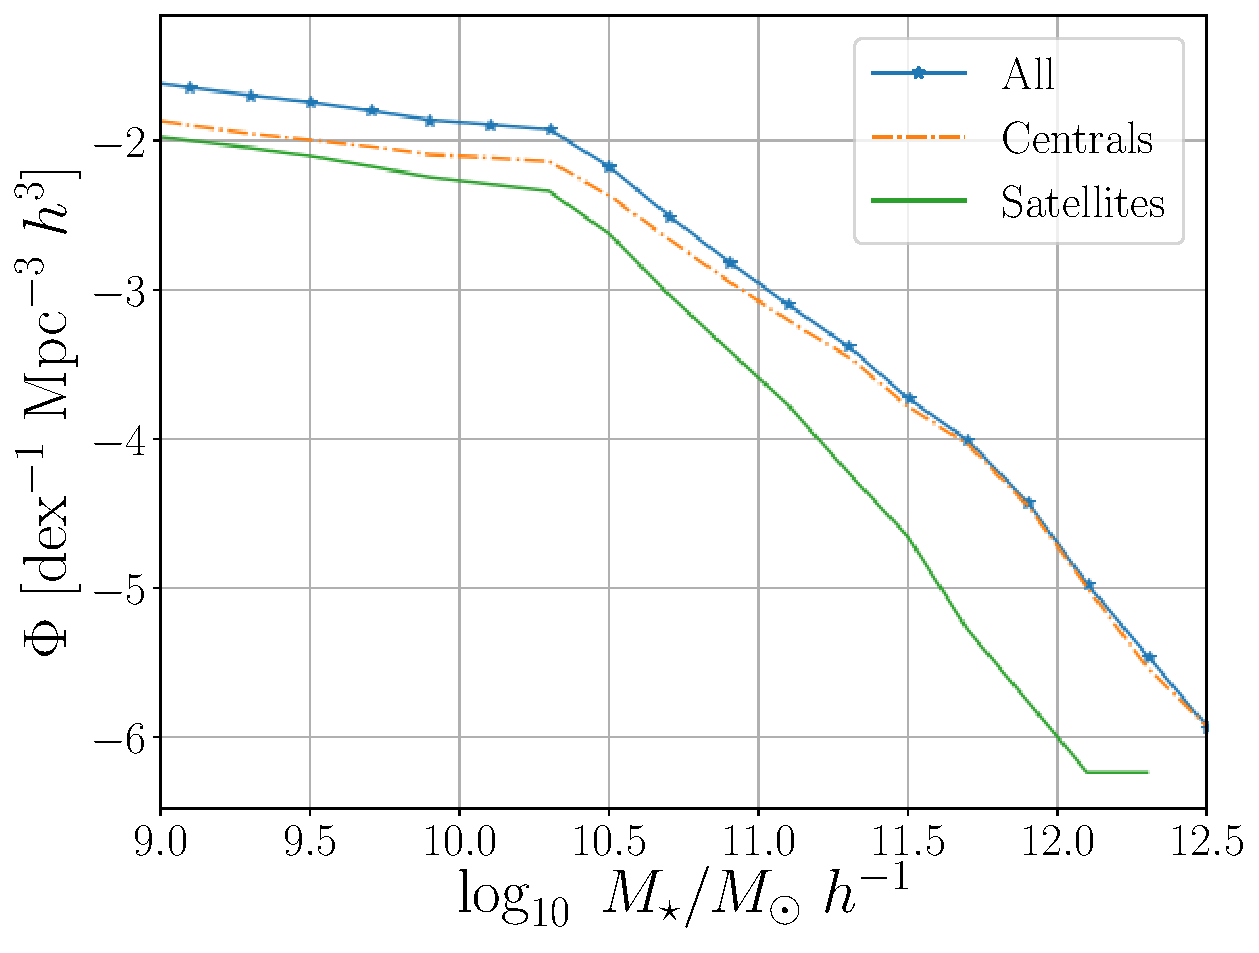
\includegraphics[width=1\columnwidth]{figuras/Histogramas.pdf}
    \caption{Stellar mass functions for all galaxies and their partition
      into centrals and satellites. 
    Although the mass resolution in TNG300-1 resolves individual
    galaxies below $10^{9}$ \Msunh we use this value as a threshold
    because galaxies above this mass has an appropriate resolution in
    the formation history to estimate their assembly time.}
    \label{fig:stellar_fuction}
\end{figure}


\begin{figure}
    \centering
     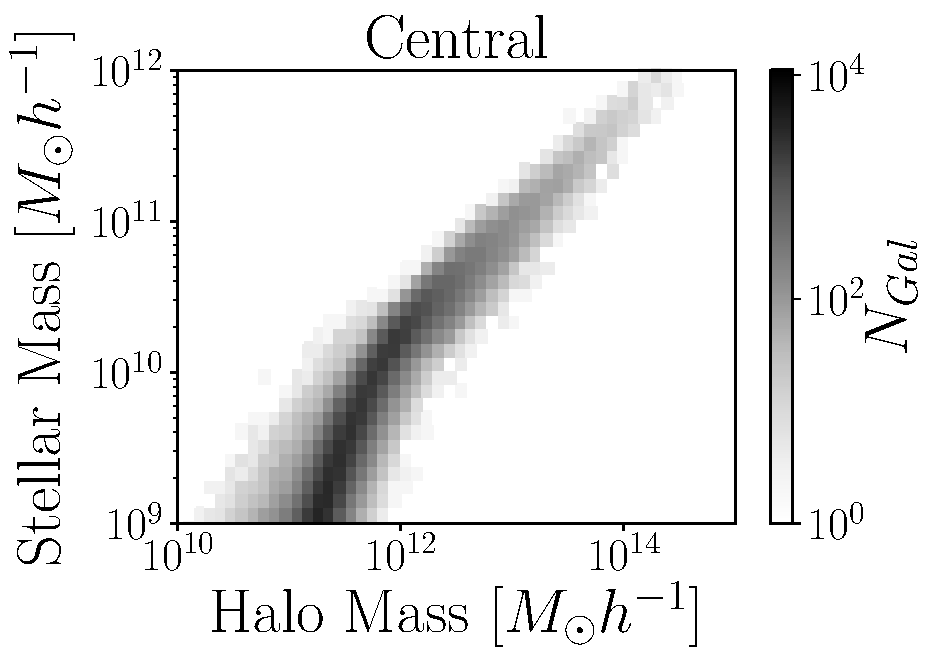
\includegraphics[width=1\columnwidth]{figuras/his2_centrales.pdf}
    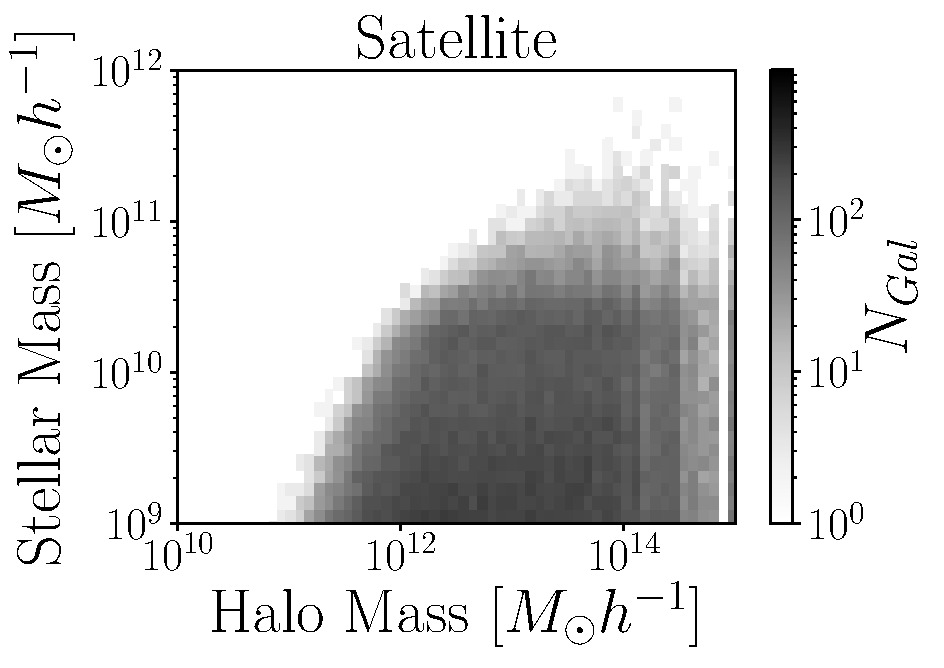
\includegraphics[width=1\columnwidth]{figuras/his2_satelite.pdf}
    \caption{Relationship between stellar mass and the parent dark
      matter halo mass for central and satellite galaxies.} 
    \label{fig:stellar_to_halo}
\end{figure}


\begin{figure}
    \centering
    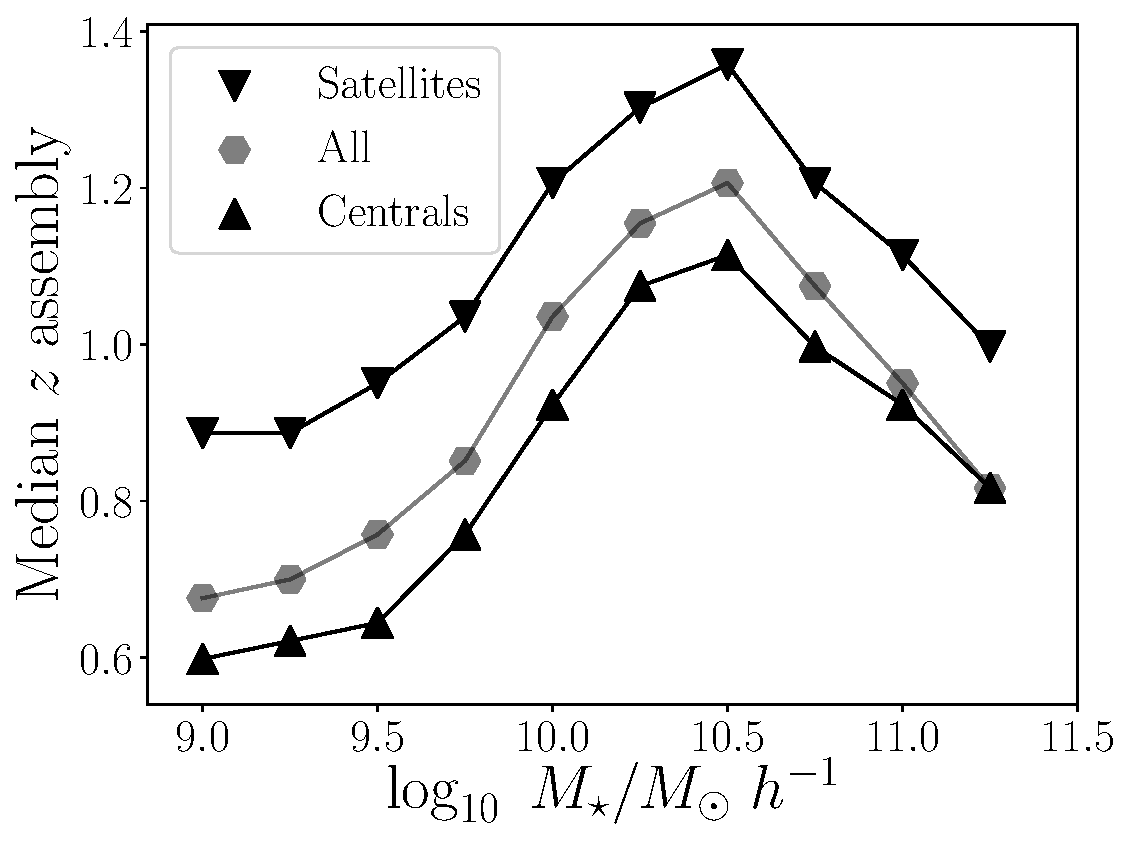
\includegraphics[width=1\columnwidth]{figuras/median_assembly.pdf}
    \caption{Median redshift of assembly as a function of stellar mass.
    Different symbols correspond to satellites, centrals or all galaxies.
    The stellar mass around $10^{10.5}$\Msunh shows a transition between two 
    regimes of \emph{upsizing} and \emph{downsizing}.}
    \label{fig:median_assembly}
\end{figure}


Subhalos and galaxies were identified using SUBFIND algorithm.
We use the baryonic merger trees to estimate the assembly time for the
galaaxies.
These trees were constructed using the SUBLINK algorithm at the
subhalo level \citep{2015MNRAS.449...49R}.

We take as the stellar mass the measurement within
twice the stellar half mass radius of each subhalo.
We only use galaxies with stellar masses at $z=0$ greater than
$10^{9}$\Msunh.
With this selection we end up with close to 128 thousand galaxies.
This allows us to have galaxies with a well resolved formation
history. 
Galaxies above this treshold are resolved with at least $150$ stellar
particles. 

We extract the main branch of the tree by following back at every
snapshot the most massive progenitor.
We use this main branch to define the assembly time as the redshift
at which the galaxy in the branch has exactly half of its stellar mass
at $z=0$.   


Figure \ref{fig:stellar_fuction} shows the stellar mass functions for
this sample.
There we observe that the most massive satellite galaxy has a stellar
mass of $\approx 10^{12}$\Msunh.    
We note that there are approximately $20$ central galaxies
with a similar mass.
In this Letter we measure correlations functions on central and
satellites in different mass bins.
For this reason we impose a  minimum of $1000$ galaxies
in a mass bin of $0.25$ dex in width to have a reasonable
measurement. 
This limits translates into in having an an upper mass limit of
$10^{11.5}$\Msunh, even though there are galaxies in the simulation
more massive than this value.

Figure \ref{fig:stellar_to_halo} shows the stellar mass as a function
of the DM halo mass of the host.
The panels split the galaxies intro centrals and satellites. 
This shows us that centrals follow a relatively tight relationship
between stellar mass and DM halo mass.
On the other hand, satallite galaxies do not follow a clear trend.
For instance, satellite galaxies with stellar masses $\approx
10^{9}$\Msunh are hosted by halos with masses that span almost three
orders of magnitude.

Figure \ref{fig:median_assembly} summarizes the trends for the
assembly times as a function of mass for central and satellite
galaxies.
From that Figure we see that, at fixed stellar mass, central galaxies
assembly later than  satellite galaxies.
Apart from this systematic offset the trend with stellar mass is
similar for centrals and satellites.
The main trend is characterized by a transitional stellar mass around 
$\approx 3\times 10^{10}$ \Msunh.
This stellar mass presents the earliest assembly times, always above $z=1$.
Above that mass, more massive galaxies assembly later; below that
value more massive galaxies assembly earlier.

In what follows we dissect the assembly time distribution into
early/late assembly to quantify how those differences translate into
different clustering strenght.
We define early assemblying galaxies as those falling into the
quartile with the highest assembly redshifts while late assemblying
galaxies fall into the quartile with the lowest assembly redshifts.
In order to explore observational proxies for the assembly time we
also split our samples into quartiles for the specific star formation
rate (sSFR) and $(g-i)$ colour. 

\section{Clustering dependence on assembly time}
\label{sec:results}

\begin{figure*}
    \centering
    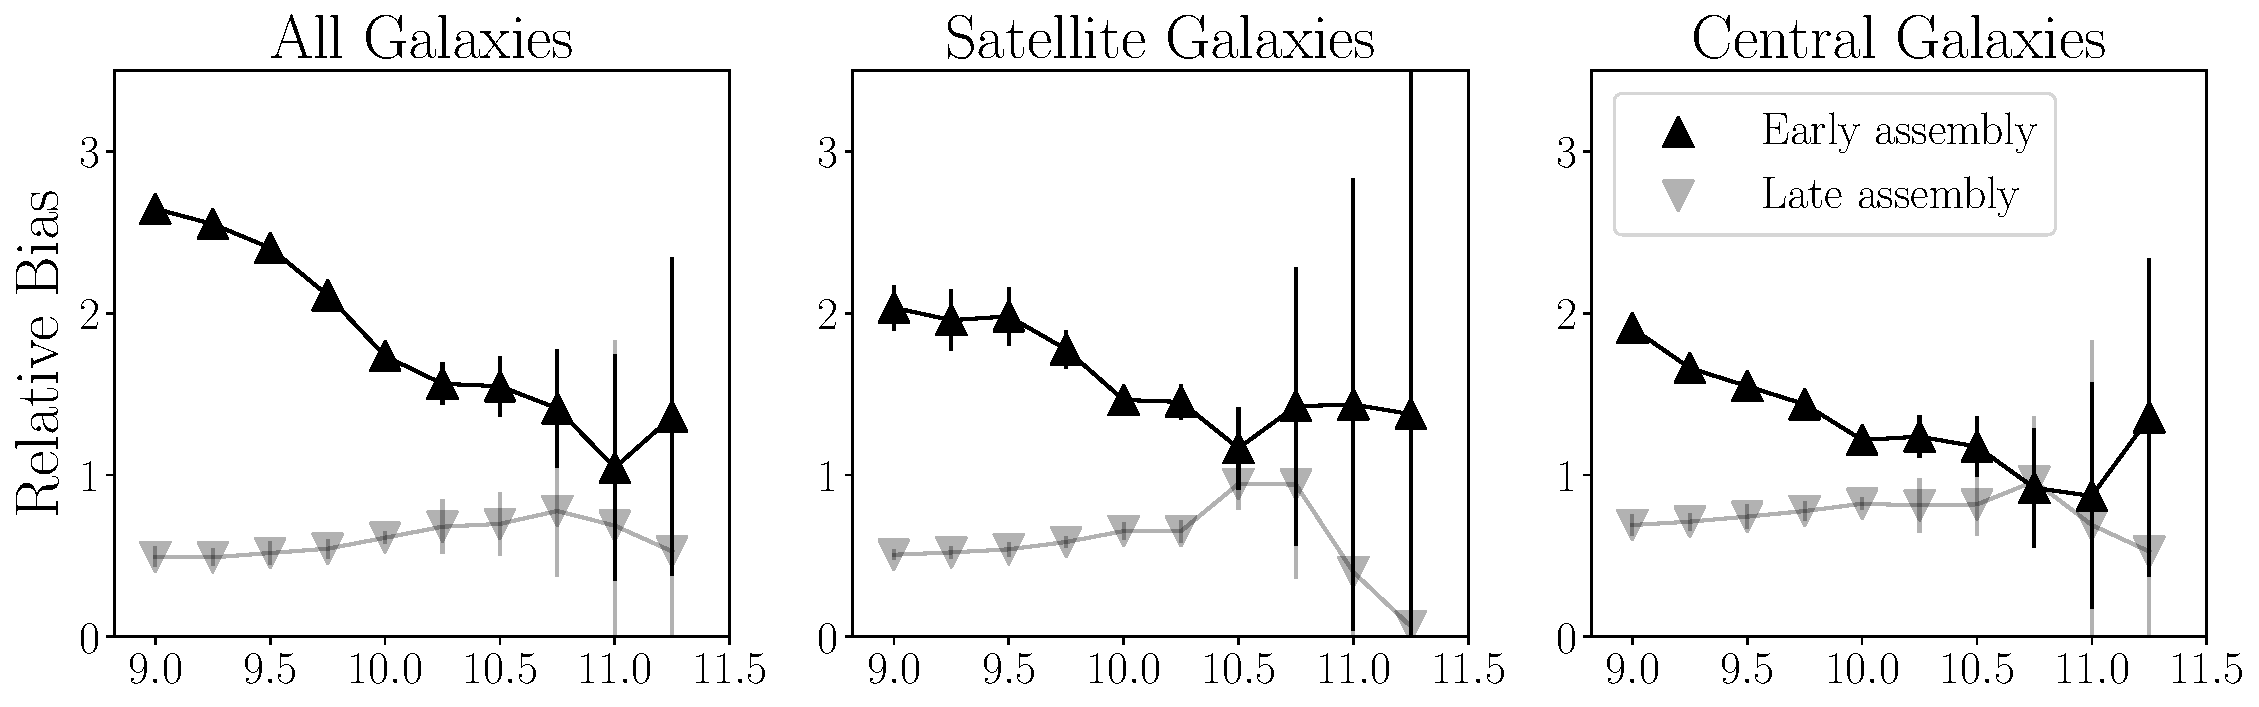
\includegraphics[width=1.8\columnwidth]{figuras/bias_galaxies.pdf}
    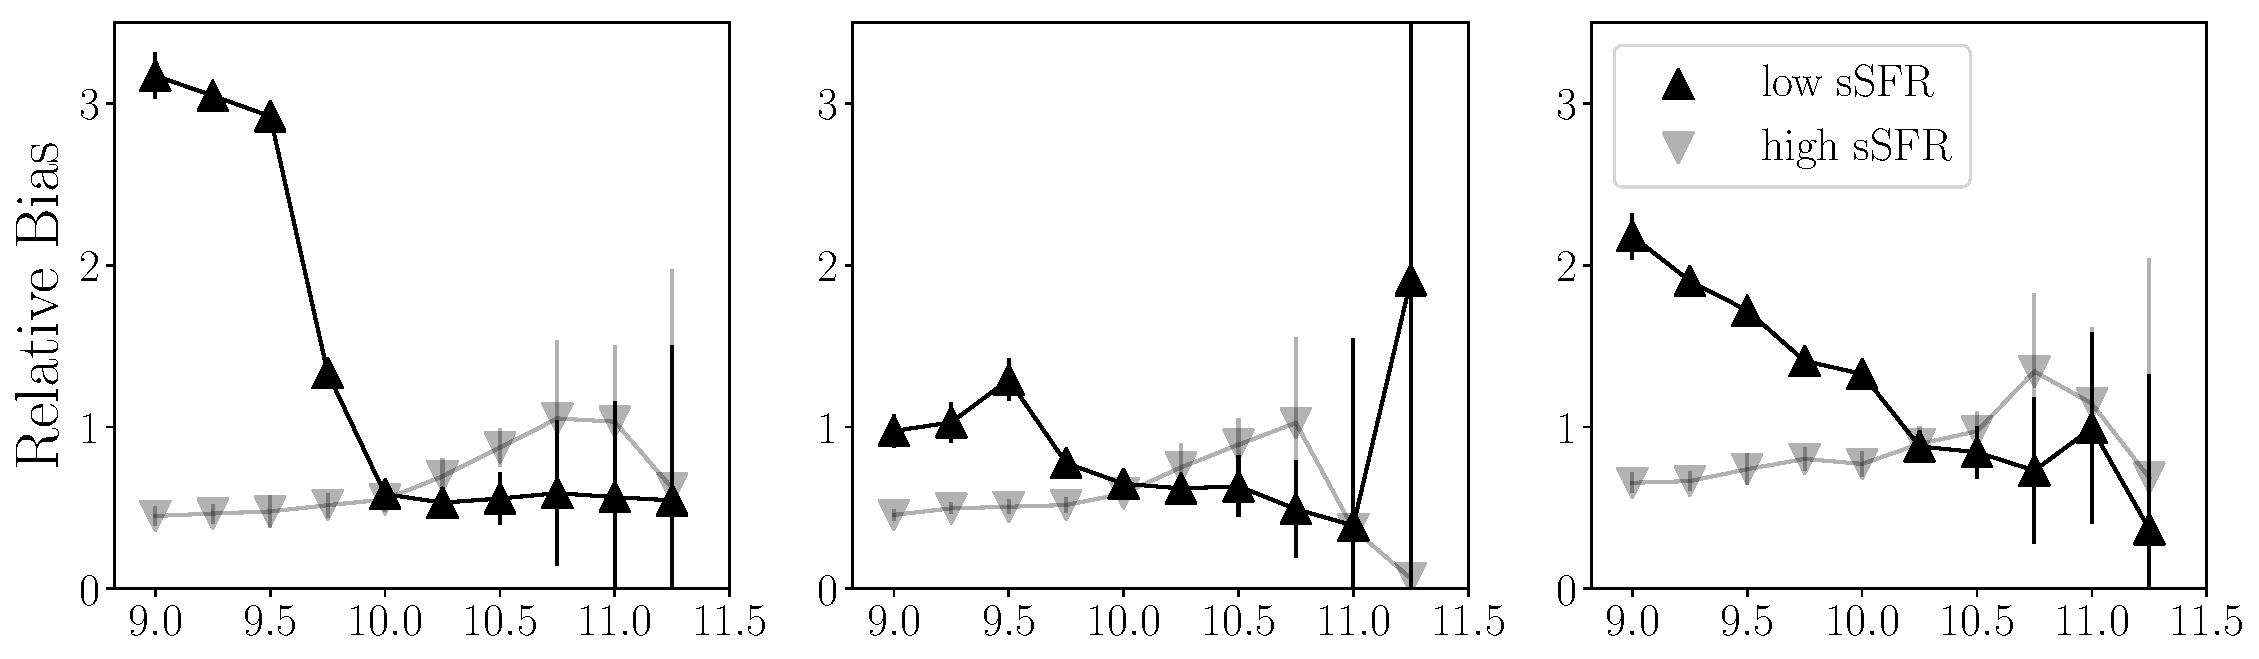
\includegraphics[width=1.8\columnwidth]{figuras/ssfr_bias_galaxies.pdf}
    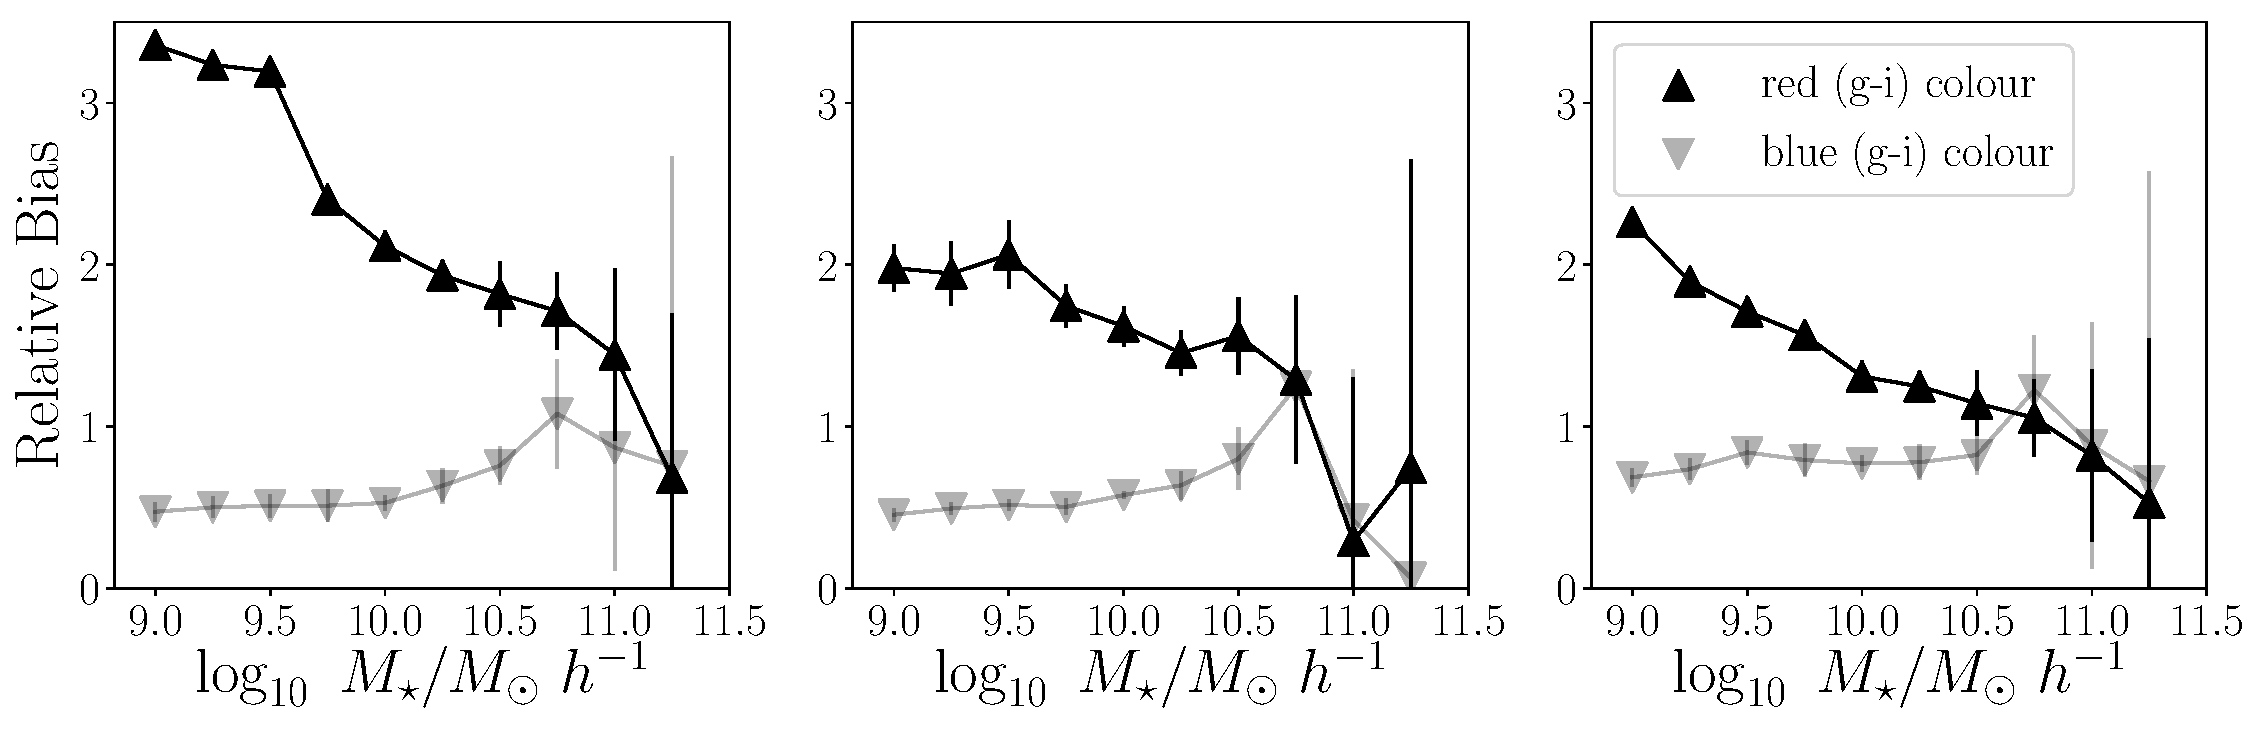
\includegraphics[width=1.8\columnwidth]{figuras/color_bias_galaxies.pdf}
    \caption{Relative galaxy bias as a function of stellar mass.
    We consider separately all galaxies, satellites and centrals.
    The bias is higher for early assembling galaxies (upper row).
    The relative bias results cannot be reproduced with cuts in the
    specific star formation rate (middle row), while cuts in the
    $(g-i)$ colour (lower row) reproduce the main trends obtained with
    assembly time cuts.}
    \label{fig:galaxy_bias}
\end{figure*}

\begin{figure*}
    \centering
    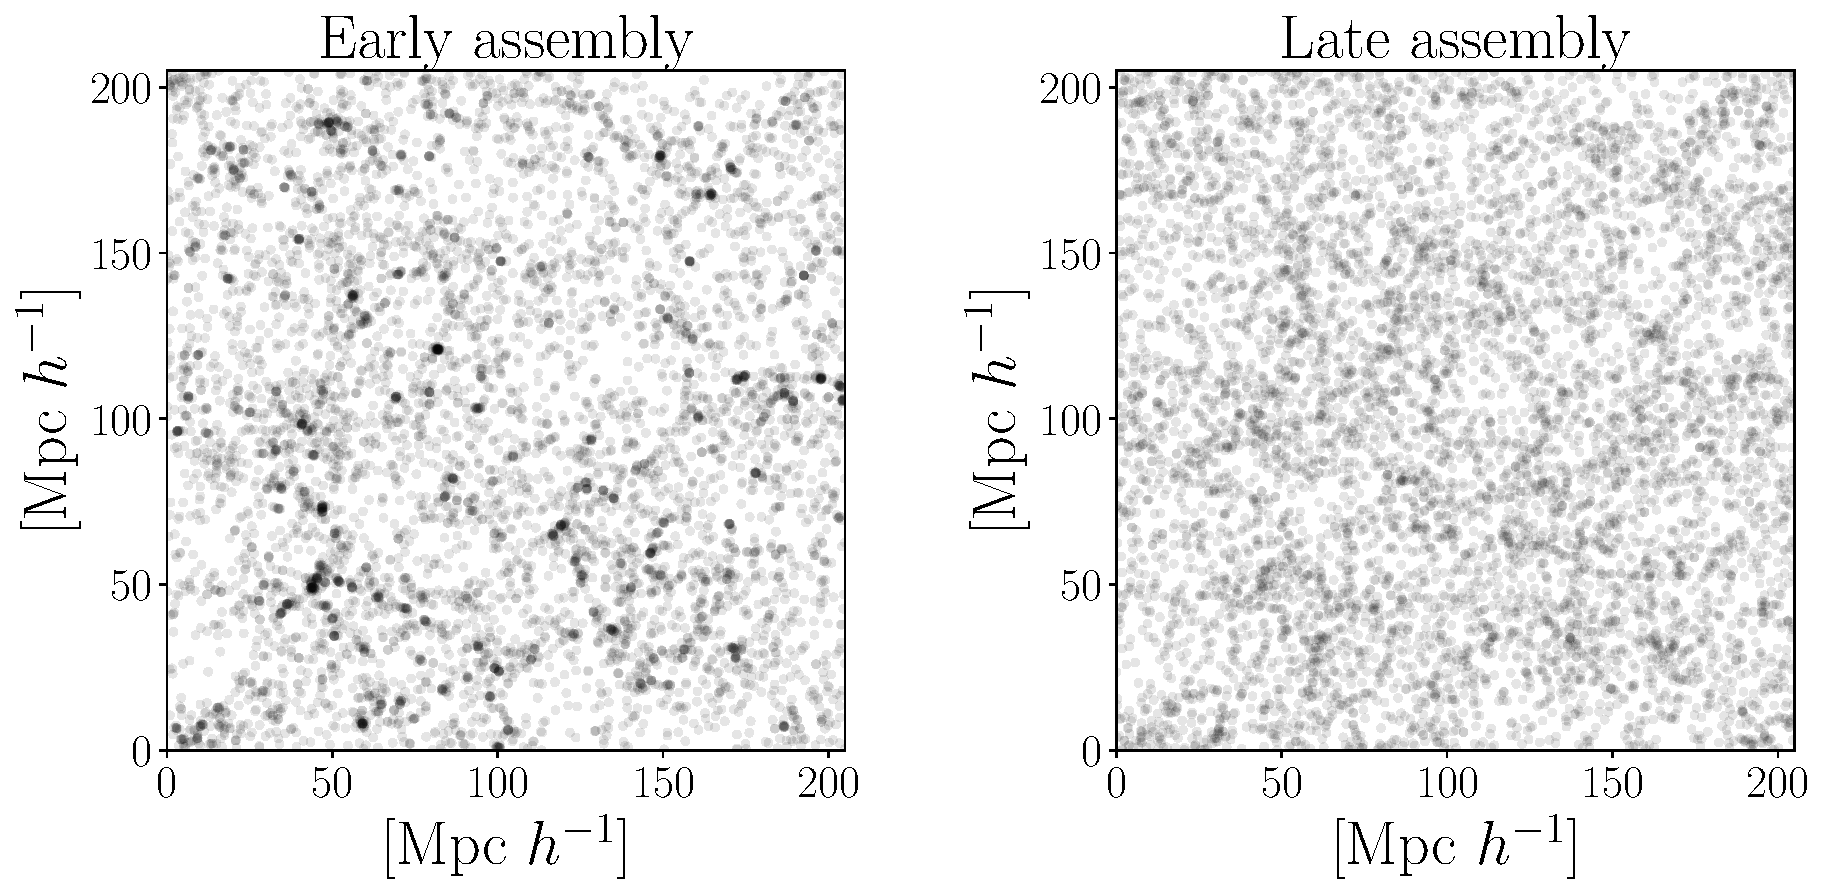
\includegraphics[width=1.6\columnwidth]{figuras/scatter_assembly.pdf}
%    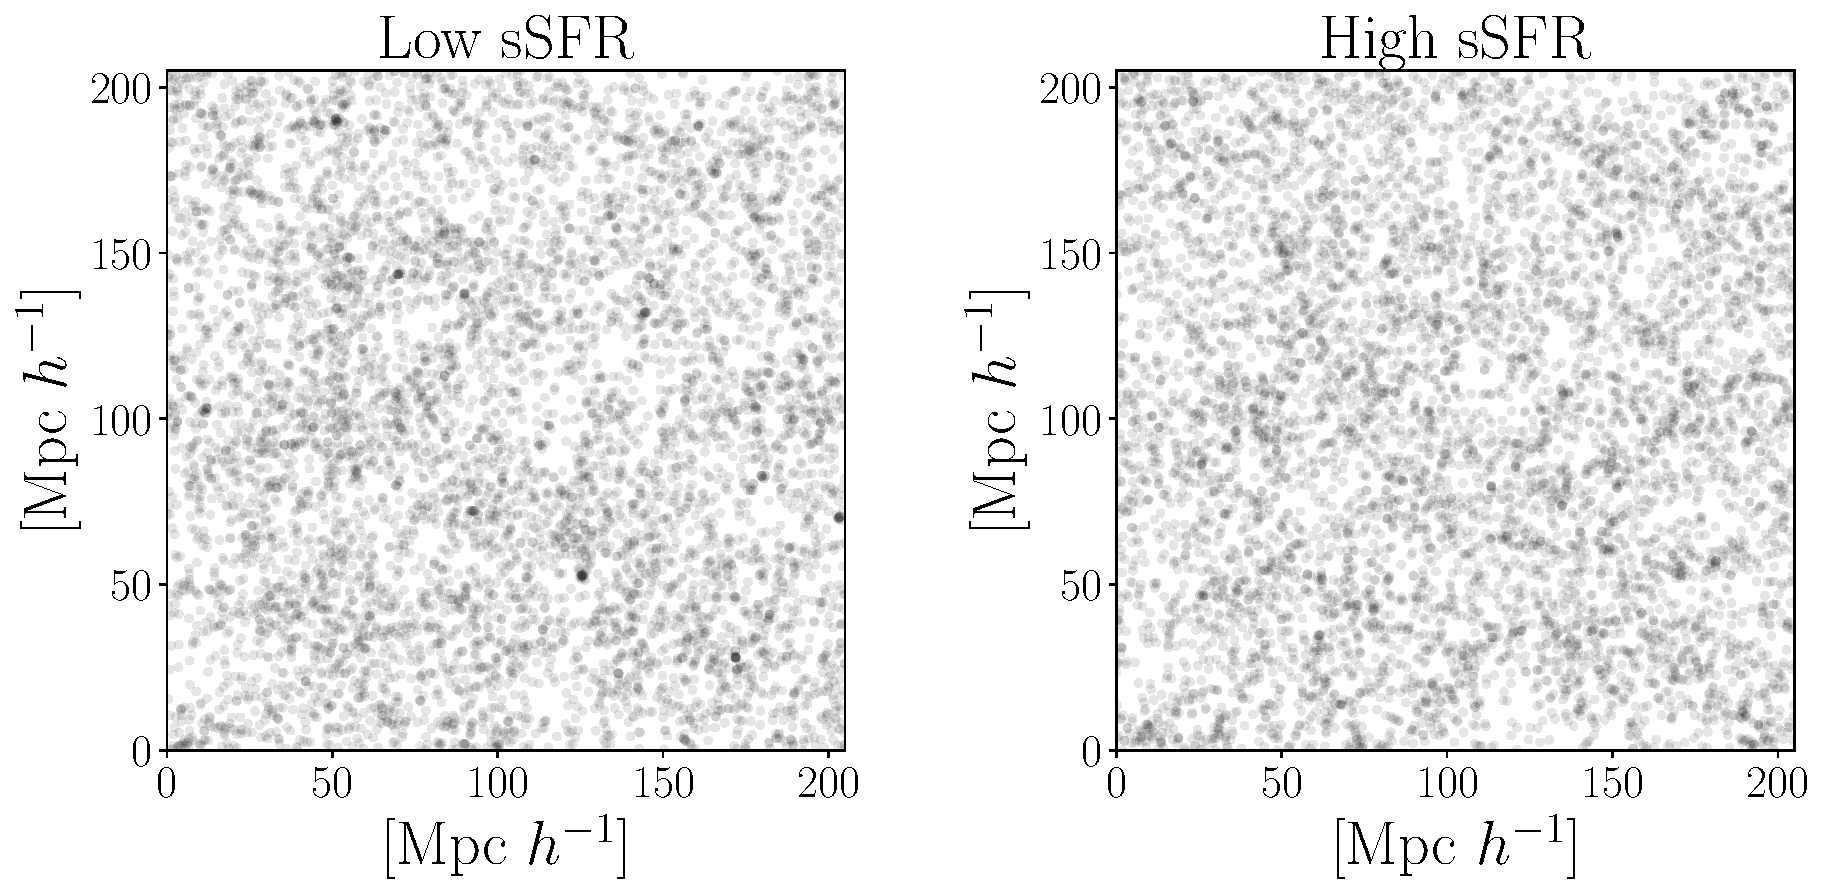
\includegraphics[width=1.6\columnwidth]{figuras/scatter_ssfr.pdf}
    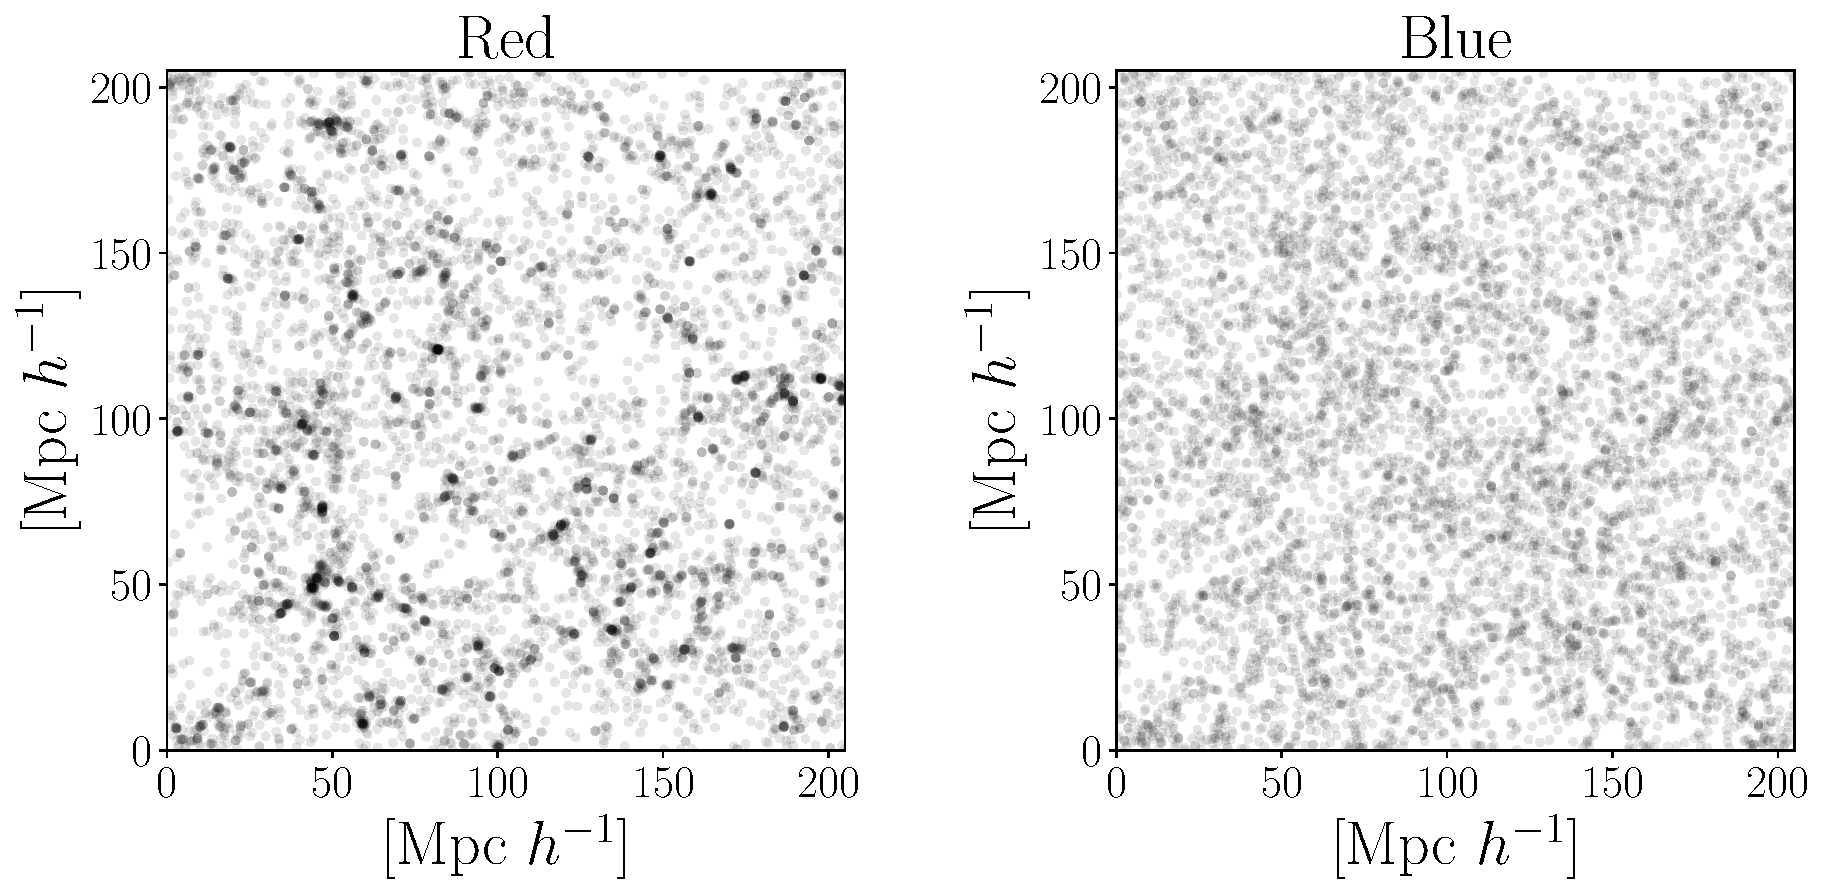
\includegraphics[width=1.6\columnwidth]{figuras/scatter_color.pdf}
    \caption{Comparison of the spatial distribution of galaxies with 
      \emph{early}/\emph{late} assembly and \emph{red}/\emph{blue}
      $(g-r)$ colours.
      The galaxies included in the plot have stellar masses around
      $10^{10}$\Msunh.  
      Each panel projects all the galaxy positions over the $x$-$y$
      plane.  
    Each panel has $\sim7$k galaxies. }
    \label{fig:comparison}
\end{figure*}


We follow \cite{2020MNRAS.tmp.1844M} to quantify the changes in galaxy
clustering we estimate the relative galaxy bias by taking the ratio of
the 2-point correlation function of two samples: 
%
\begin{equation}
b_r(r, S|A)= \frac{\xi_S(r)}{\xi_A(r)}, 
\label{eq:relative}
\end{equation}
%
where $\xi_A$ corresponds to the correlation function from a general
sample $A$ that includes all the galaxies in a fixed stellar mass bin,
while $\xi_S$ is the correlation function computed for a sub-sample,
$S$, of galaxies in $A$. 
In our case the sub-samples are built from either the first and last
quartile in the redshift assembly distribution. 


We compute the correlation function in the separation range of
$5$ \Mpch\ to $10$ \Mpch\ split into $10$ linearly spaced bins. 
The relative bias is computed over every bin.
We report the mean value of that ratio and we associate an error bar
to using the standard deviation over the same separation bins.

Figure \ref{fig:galaxy_bias} summarizes the main result of this Letter.
There we present the relative galaxy bias as a
function of stellar mass for central, satellites, and all galaxies
separately. 
The upper, middle and lower rows correspond to splits on the assembly
time, specific star formation rate and colour, respectively.
The relative bias for early assembly galaxies is higher in comparison
with the later assembly galaxies.
The clustering difference between early and late assemblying galaxies
is more pronounced towards lower masses below $5 \times 10^{10}$
\Msunh.
Above that mass the large error bars do not allow for a confident
assesment. 
The assembly bias holds with similar strength both for satellites and
centrals. 
The transitional mass below which the effect is the noticeable is also
similar, close to $5\times 10^{10}$\Msunh.

Using the sSFR produces a similar picture but quite different in the
details. 
For the general galaxy population the assembly bias effect is
noticeable for masses below $10^{10}$\Msunh; the effect is weaker for
satellite galaxies than it is for centrals. 
In contrast, the split in $(g-r)$ colour produces results that
closely follow the assembly time cuts both in the effect amplitud and
its mass trends.

Figure \ref{fig:comparison} provides a qualitative summary of the main
result in this Letter.
The points correspond to galaxies (centrals and satellites combined) 
within the same mass bin around $10^{10}$\Msunh. 
In the upper row galaxies are split following their assembly time,
while in the lower row they are split red and blue $(g-r)$ colours.
Early assemblying galaxies are clustered more strongly than late
assemblying galaxies. 
The clustering differences are well approximated by splits into
red/blue galaxies. 



\section{Discussion and conclusions}
\label{sec:conclu}

In this Letter we used an state-of-the-art hydro-dynamical simulation
to study how the clustering of galaxies depends on their assembly
time.
We performed the analysis in the mass range $10^{9}$\Msunh $\leq
M_{\star} \leq 10^{11.5}$ for the whole galaxy population and
separately for centrals and satellites.

Using the 2-point correlation function, 
we computed the relative bias to  quantified the clustering-age
dependence for galaxies at fixed stellar mass.
Early-assembly galaxies tend to be more clustered than late-assembly galaxies.
This trend is stronger towards lower stellar masses below a mass
treshold of $(6\pm1)\times 10^{10}$ \Msunh.  
The strengt of the relative bias is similar for satellites and
centrals. 
We showed that the specific star formation cuts cannot reproduce those
trends, while the $(g-r)$ colour cuts can. 

Our results could be observationally verified with a high degree of
accuracy with the Dark Energy Spectroscopic Instrument (DESI).
DESI includes a Bright Galaxy Survey that will take spectra of
10 million galaxies.
It will including targets with an apparent $r$-band magnitude brighter
than $19.5$, approximately 2 magnitudes deeper than the SDSS
main survey.  
This means that DESI will produce a complete survey for galaxies with
stellar masses $10^{9}$\Msunh within a distance of $\approx 200$
\Mpch. 


\section*{Data availability}
The datasets were derived from sources in the public domain
\url{https://www.tng-project.org/data/}. 


\bibliographystyle{mnras}
\bibliography{bibliography.bib}


% Don't change these lines
\bsp	% typesetting comment
\label{lastpage}
\end{document}
